

\subsection{Specifying Coordinates\\指定坐标}

Karl now wants to add the sine and cosine lines. He knows already that he can
use the |color=| option to set the lines' colors. So, what is the best way to
specify the coordinates?

现在Karl想要添加正弦和余弦线。他已经知道可以使用|color=|选项来设置线条的颜色。那么,最好的方法是如何指定坐标呢?



There are different ways of specifying coordinates. The easiest way is to say
something like |(10pt,2cm)|. This means 10pt in $x$-direction and 2cm in
$y$-directions. Alternatively, you can also leave out the units as in |(1,2)|,
which means ``one times the current $x$-vector plus twice the current
$y$-vector''. These vectors default to 1cm in the $x$-direction and 1cm in the
$y$-direction, respectively.

有不同的指定坐标的方法。最简单的方法是使用类似于|(10pt,2cm)|的表示方式。这表示在$x$方向上为10pt,在$y$方向上为2cm。另外,你也可以省略单位,例如|(1,2)|,它表示``当前$x$向量的一倍加上当前$y$向量的两倍''。这些向量默认分别为1cm和1cm。

In order to specify points in polar coordinates, use the notation |(30:1cm)|,
which means 1cm in direction 30 degree. This is obviously quite useful to ``get
to the point $(\cos 30^\circ,\sin 30^\circ)$ on the circle''.

为了指定极坐标中的点,可以使用|(30:1cm)|的表示方式,它表示方向为30度的1cm。这显然非常有用,可以``到达圆上的点$(\cos 30^\circ,\sin 30^\circ)$''。

% 极坐标是表示平面上的点的一种坐标系统。

% 极坐标将平面上的每个点表示成(r,θ)的形式,其中:

% r是该点到坐标原点的距离,叫做极径。

% θ是该点在平面上的角度,叫做极角。

% 极角θ的取值范围通常是[0, 2π),也可以是[0, 360°)。θ=0对应正右方。

% 极坐标与笛卡尔坐标的转换关系为:

% x = rcosθ

% y = rsinθ

% 极坐标的性质和应用包括:

% 极坐标通过距离原点和角度唯一确定一个点。

% 极坐标对于表示圆、螺线等曲线方便。

% 极坐标可用于表示向心力和离心力问题。

% 极坐标可简化表达微分方程的解析解。

% 极坐标在计算机图形学中也有应用。

% 极坐标结合复数的指数形式,可以表示复平面上的点。

% 总之,极坐标是除了笛卡尔坐标以外描述平面点的重要方法。它在某些问题中表达更简洁和直观。但笛卡尔坐标对于表示直线方程更方便。两者都有各自的优点。

You can add a single |+| sign in front of a coordinate or two of them as in
|+(0cm,1cm)| or |++(2cm,0cm)|. Such coordinates are interpreted differently:
The first form means ``1cm upwards from the previous specified position'' and
the second means ``2cm to the right of the previous specified position, making
this the new specified position''. For example, we can draw the sine line as
follows:
%

你可以在坐标前面加一个单独的|+|符号,或者两个|+|符号,例如|+(0cm,1cm)|或|++(2cm,0cm)|。这些坐标的解释方式不同:第一种形式表示相对于之前指定的位置向上移动1cm'',而第二种表示相对于之前指定的位置向右移动2cm,并将其作为新指定的位置''。例如,我们可以如下绘制正弦线:

\begin{codeexample}[]
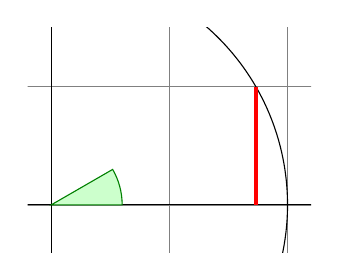
\begin{tikzpicture}[scale=3]
  \clip (-0.1,-0.2) rectangle (1.1,0.75);
  \draw[step=.5cm,gray,very thin] (-1.4,-1.4) grid (1.4,1.4);
  \draw (-1.5,0) -- (1.5,0);
  \draw (0,-1.5) -- (0,1.5);
  \draw (0,0) circle [radius=1cm];
  \filldraw[fill=green!20,draw=green!50!black] (0,0) -- (3mm,0mm)
      arc [start angle=0, end angle=30, radius=3mm] -- cycle;
  \draw[red,very thick] (30:1cm) -- +(0,-0.5);
\end{tikzpicture}
\end{codeexample}

Karl used the fact $\sin 30^\circ = 1/2$. However, he very much doubts that his
students know this, so it would be nice to have a way of specifying ``the point
straight down from |(30:1cm)| that lies on the $x$-axis''. This is, indeed,
possible using a special syntax: Karl can write \verb!(30:1cm |- 0,0)!. In
general, the meaning of |(|\meta{p}\verb! |- !\meta{q}|)| is ``the intersection
of a vertical line through $p$ and a horizontal line through $q$''.

Karl事实上使用了$\sin 30^\circ = 1/2$。然而,他非常怀疑他的学生们是否知道这一点,所以最好有一种方法来指定从|(30:1cm)|指向$x$轴下方的点''。事实上,使用一种特殊的语法是可以实现的:Karl可以写成\verb!(30:1cm |- 0,0)!。一般来说,|(|\meta{p}\verb! |- !\meta{q}|)|的意思是通过$p$的垂直线与$q$的水平线的交点''。
%%% todo 这段需要再看看

Next, let us draw the cosine line. One way would be to say
\verb!(30:1cm |- 0,0) -- (0,0)!. Another way is the following: we ``continue''
from where the sine ends:
%

接下来,让我们绘制余弦线。一种方式是\verb!(30:1cm |- 0,0) -- (0,0)!。另一种方式是:我们``延续''正弦线的结束位置:

\begin{codeexample}[]
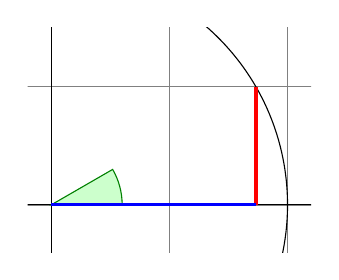
\begin{tikzpicture}[scale=3]
  \clip (-0.1,-0.2) rectangle (1.1,0.75);
  \draw[step=.5cm,gray,very thin] (-1.4,-1.4) grid (1.4,1.4);
  \draw (-1.5,0) -- (1.5,0);
  \draw (0,-1.5) -- (0,1.5);
  \draw (0,0) circle [radius=1cm];
  \filldraw[fill=green!20,draw=green!50!black] (0,0) -- (3mm,0mm)
      arc [start angle=0, end angle=30, radius=3mm] -- cycle;
  \draw[red,very thick]  (30:1cm) -- +(0,-0.5);
  \draw[blue,very thick] (30:1cm) ++(0,-0.5) -- (0,0);
\end{tikzpicture}
\end{codeexample}

Note that there is no |--| between |(30:1cm)| and |++(0,-0.5)|. In detail, this
path is interpreted as follows: ``First, the |(30:1cm)| tells me to move my pen
to $(\cos 30^\circ,1/2)$. Next, there comes another coordinate specification,
so I move my pen there without drawing anything. This new point is half a unit
down from the last position, thus it is at $(\cos 30^\circ,0)$. Finally, I move
the pen to the origin, but this time drawing something (because of the |--|).''

请注意,在 |(30:1cm)| 和 |++(0,-0.5)| 之间没有 |--|。具体来说,该路径的解释如下:"首先,|(30:1cm)| 告诉我将笔移动到 $(\cos 30^\circ,1/2)$。接下来,出现了另一个坐标指定,所以我将笔移动到那个位置,但不画任何东西。这个新点相对于上一个位置向下移动了半个单位,因此它位于 $(\cos 30^\circ,0)$。最后,我将笔移动到原点,但这次画了一些东西(因为有 |--|)"。



To appreciate the difference between |+| and |++| consider the following
example:


为了理解 |+| 和 |++| 之间的区别,请考虑以下示例:%todo 后面再看看...
%
\begin{codeexample}[]

\begin{tikzpicture}
  \def\rectanglepath{-- ++(1cm,0cm)  -- ++(0cm,1cm)  -- ++(-1cm,0cm) -- cycle}
  \draw (0,0) \rectanglepath;
  \draw (1.5,0) \rectanglepath;
\end{tikzpicture}
\end{codeexample}

By comparison, when using a single |+|, the coordinates are different:
%

相比之下,当使用单个 |+| 时,坐标是不同的:

\begin{codeexample}[]

\begin{tikzpicture}
  \def\rectanglepath{-- +(1cm,0cm)  -- +(1cm,1cm)  -- +(0cm,1cm) -- cycle}
  \draw (0,0) \rectanglepath;
  \draw (1.5,0) \rectanglepath;
\end{tikzpicture}
\end{codeexample}


Naturally, all of this could have been written more clearly and more
economically like this (either with a single or a double |+|):

当然,所有这些都可以更清晰、更简洁地写成这样(无论是使用单个还是双个 |+|):

\begin{codeexample}[]
\tikz \draw (0,0) rectangle +(1,1)  (1.5,0) rectangle +(1,1);
\end{codeexample}





\mshowc{section}
\mshowc{subsection}
\mshowc{subsubsection}
\end{document}

\subsection{Intersecting Paths}

Karl is left with the line for $\tan \alpha$, which seems difficult to specify
using transformations and polar coordinates. The first -- and easiest -- thing
he can do is so simply use the coordinate |(1,{tan(30)})| since \tikzname's
math engine knows how to compute things like |tan(30)|. Note the added braces
since, otherwise, \tikzname's parser would think that the first closing
parenthesis ends the coordinate (in general, you need to add braces around
components of coordinates when these components contain parentheses).

Karl can, however, also use a more elaborate, but also more ``geometric'' way
of computing the length of the orange line: He can specify intersections of
paths as coordinates. The line for $\tan \alpha$ starts at $(1,0)$ and goes
upward to a point that is at the intersection of a line going ``up'' and a line
going from the origin through |(30:1cm)|. Such computations are made available
by the |intersections| library.

What Karl must do is to create two ``invisible'' paths that intersect at the
position of interest. Creating paths that are not otherwise seen can be done
using the |\path| command without any options like |draw| or |fill|. Then, Karl
can add the |name path| option to the path for later reference. Once the paths
have been constructed, Karl can use the |name intersections| to assign names to
the coordinate for later reference.
%
\begin{codeexample}[code only]
\path [name path=upward line] (1,0) -- (1,1);
\path [name path=sloped line] (0,0) -- (30:1.5cm); % a bit longer, so that there is an intersection

% (add `\usetikzlibrary{intersections}' after loading tikz in the preamble)
\draw [name intersections={of=upward line and sloped line, by=x}]
  [very thick,orange] (1,0) -- (x);
\end{codeexample}


\subsection{Adding Arrow Tips}

Karl now wants to add the little arrow tips at the end of the axes. He has
noticed that in many plots, even in scientific journals, these arrow tips seem
to be missing, presumably because the generating programs cannot produce them.
Karl thinks arrow tips belong at the end of axes. His son agrees. His students
do not care about arrow tips.

It turns out that adding arrow tips is pretty easy: Karl adds the option |->|
to the drawing commands for the axes:
%
\begin{codeexample}[preamble={\usetikzlibrary{intersections}}]
\begin{tikzpicture}[scale=3]
  \clip (-0.1,-0.2) rectangle (1.1,1.51);
  \draw[step=.5cm,gray,very thin] (-1.4,-1.4) grid (1.4,1.4);
  \draw[->] (-1.5,0) -- (1.5,0);
  \draw[->] (0,-1.5) -- (0,1.5);
  \draw (0,0) circle [radius=1cm];
  \filldraw[fill=green!20,draw=green!50!black] (0,0) -- (3mm,0mm)
        arc [start angle=0, end angle=30, radius=3mm] -- cycle;
  \draw[red,very thick]    (30:1cm) -- +(0,-0.5);
  \draw[blue,very thick]   (30:1cm) ++(0,-0.5) -- (0,0);

  \path [name path=upward line] (1,0) -- (1,1);
  \path [name path=sloped line] (0,0) -- (30:1.5cm);
  \draw [name intersections={of=upward line and sloped line, by=x}]
        [very thick,orange] (1,0) -- (x);
\end{tikzpicture}
\end{codeexample}

If Karl had used the option |<-| instead of |->|, arrow tips would have been
put at the beginning of the path. The option |<->| puts arrow tips at both ends
of the path.

There are certain restrictions to the kind of paths to which arrow tips can be
added. As a rule of thumb, you can add arrow tips only to a single open
``line''. For example, you cannot add tips to, say, a rectangle or a circle.
However, you can add arrow tips to curved paths and to paths that have several
segments, as in the following examples:
%
\begin{codeexample}[]
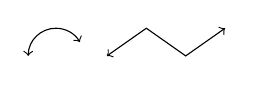
\begin{tikzpicture}
  \draw [<->] (0,0) arc [start angle=180, end angle=30, radius=10pt];
  \draw [<->] (1,0) -- (1.5cm,10pt) -- (2cm,0pt) -- (2.5cm,10pt);
\end{tikzpicture}
\end{codeexample}

Karl has a more detailed look at the arrow that \tikzname\ puts at the end. It
looks like this when he zooms it: \tikz[baseline] \draw[->,line width=1pt]
(0pt,.5ex) -- ++(10pt,0pt);. The shape seems vaguely familiar and, indeed, this
is exactly the end of \TeX's standard arrow used in something like $f\colon A
\to B$.

Karl likes the arrow, especially since it is not ``as thick'' as the arrows
offered by many other packages. However, he expects that, sometimes, he might
need to use some other kinds of arrow. To do so, Karl can say |>=|\meta{kind of
end arrow tip}, where \meta{kind of end arrow tip} is a special arrow tip
specification. For example, if Karl says |>=Stealth|, then he tells \tikzname\
that he would like  ``stealth-fighter-like'' arrow tips:
\todosp{remaining instance of bug \#473}
%
\begin{codeexample}[preamble={\usetikzlibrary{arrows.meta}}]
\begin{tikzpicture}[>=Stealth]
  \draw [->] (0,0) arc [start angle=180, end angle=30, radius=10pt];
  \draw [<<-,very thick] (1,0) -- (1.5cm,10pt) -- (2cm,0pt) -- (2.5cm,10pt);
\end{tikzpicture}
\end{codeexample}

Karl wonders whether such a military name for the arrow type is really
necessary. He is not really mollified when his son tells him that Microsoft's
PowerPoint uses the same name. He decides to have his students discuss this at
some point.

In addition to |Stealth| there are several other predefined kinds of arrow tips
Karl can choose from, see Section~\ref{section-arrows}. Furthermore, he can
define arrows types himself, if he needs new ones.


\subsection{Scoping}

Karl saw already that there are numerous graphic options that affect how paths
are rendered. Often, he would like to apply certain options to a whole set of
graphic commands. For example, Karl might wish to draw three paths using a
|thick| pen, but would like everything else to be drawn ``normally''.

If Karl wishes to set a certain graphic option for the whole picture, he can
simply pass this option to the |\tikz| command or to the |{tikzpicture}|
environment (Gerda would pass the options to |\tikzpicture| and Hans passes
them to |\starttikzpicture|). However, if Karl wants to apply graphic options
to a local group, he put these commands inside a |{scope}| environment (Gerda
uses |\scope| and |\endscope|, Hans uses |\startscope| and |\stopscope|). This
environment takes graphic options as an optional argument and these options
apply to everything inside the scope, but not to anything outside.

Here is an example:
%
\begin{codeexample}[]
\begin{tikzpicture}[ultra thick]
  \draw (0,0) -- (0,1);
  \begin{scope}[thin]
    \draw (1,0) -- (1,1);
    \draw (2,0) -- (2,1);
  \end{scope}
  \draw (3,0) -- (3,1);
\end{tikzpicture}
\end{codeexample}

Scoping has another interesting effect: Any changes to the clipping area are
local to the scope. Thus, if you say |\clip| somewhere inside a scope, the
effect of the |\clip| command ends at the end of the scope. This is useful
since there is no other way of ``enlarging'' the clipping area.

Karl has also already seen that giving options to commands like |\draw| apply
only to that command. It turns out that the situation is slightly more complex.
First, options to a command like |\draw| are not really options to the command,
but they are ``path options'' and can be given anywhere on the path. So,
instead of |\draw[thin] (0,0) -- (1,0);| one can also write
|\draw (0,0) [thin] -- (1,0);| or |\draw (0,0) -- (1,0) [thin];|; all of these
have the same effect. This might seem strange since in the last case, it would
appear that the |thin| should take effect only ``after'' the line from $(0,0)$
to $(1,0)$ has been drawn. However, most graphic options only apply to the
whole path. Indeed, if you say both |thin| and |thick| on the same path, the
last option given will ``win''.

When reading the above, Karl notices that only ``most'' graphic options apply
to the whole path. Indeed, all transformation options do \emph{not} apply to
the whole path, but only to ``everything following them on the path''. We will
have a more detailed look at this in a moment. Nevertheless, all options given
during a path construction apply only to this path.


\subsection{Transformations}

When you specify a  coordinate like |(1cm,1cm)|, where is that coordinate
placed on the page? To determine the position, \tikzname, \TeX, and
\textsc{pdf} or PostScript all apply certain transformations to the given
coordinate in order to determine the final position on the page.

\tikzname\ provides numerous options that allow you to transform coordinates in
\tikzname's private coordinate system. For example, the |xshift| option allows
you to shift all subsequent points by a certain amount:

\begin{codeexample}[]
\tikz \draw (0,0) -- (0,0.5) [xshift=2pt] (0,0) -- (0,0.5);
\end{codeexample}

It is important to note that you can change transformation ``in the middle of a
path'', a feature that is not supported by \pdf\ or PostScript. The reason is
that \tikzname\ keeps track of its own transformation matrix.

Here is a more complicated example:
%
\begin{codeexample}[]
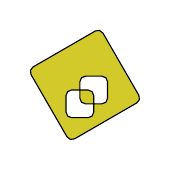
\begin{tikzpicture}[even odd rule,rounded corners=2pt,x=10pt,y=10pt]
  \filldraw[fill=yellow!80!black] (0,0)   rectangle (1,1)
        [xshift=5pt,yshift=5pt]   (0,0)   rectangle (1,1)
                    [rotate=30]   (-1,-1) rectangle (2,2);
\end{tikzpicture}
\end{codeexample}

The most useful transformations are |xshift| and |yshift| for shifting, |shift|
for shifting to a given point as in |shift={(1,0)}| or |shift={+(0,0)}| (the
braces are necessary so that \TeX\ does not mistake the comma for separating
options), |rotate| for rotating by a certain angle (there is also a
|rotate around| for rotating around a given point), |scale| for scaling by a
certain factor, |xscale| and |yscale| for scaling only in the $x$- or
$y$-direction (|xscale=-1| is a flip), and |xslant| and |yslant| for slanting.
If these transformation and those that I have not mentioned are not sufficient,
the |cm| option allows you to apply an arbitrary transformation matrix. Karl's
students, by the way, do not know what a transformation matrix is.


\subsection{Repeating Things: For-Loops}

Karl's next aim is to add little ticks on the axes at positions $-1$, $-1/2$,
$1/2$, and $1$. For this, it would be nice to use some kind of ``loop'',
especially since he wishes to do the same thing at each of these positions.
There are different packages for doing this. \LaTeX\ has its own internal
command for this, |pstricks| comes along with the powerful |\multido| command.
All of these can be used together with \tikzname, so if you are familiar with
them, feel free to use them. \tikzname\ introduces yet another command, called
|\foreach|, which I introduced since I could never remember the syntax of the
other packages. |\foreach| is defined in the package |pgffor| and can be used
independently of \tikzname, but \tikzname\ includes it automatically.

In its basic form, the |\foreach| command is easy to use:
%
\begin{codeexample}[]
\foreach \x in {1,2,3} {$x =\x$, }
\end{codeexample}

The general syntax is
|\foreach| \meta{variable}| in {|\meta{list of values}|} |\meta{commands}.
Inside the \meta{commands}, the \meta{variable} will be assigned to the
different values. If the \meta{commands} do not start with a brace, everything
up to the next semicolon is used as \meta{commands}.

For Karl and the ticks on the axes, he could use the following code:
%
\begin{codeexample}[]
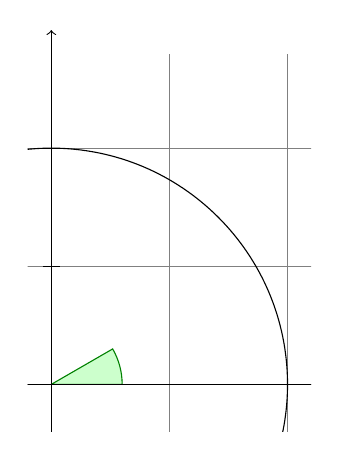
\begin{tikzpicture}[scale=3]
  \clip (-0.1,-0.2) rectangle (1.1,1.51);
  \draw[step=.5cm,gray,very thin] (-1.4,-1.4) grid (1.4,1.4);
  \filldraw[fill=green!20,draw=green!50!black] (0,0) -- (3mm,0mm)
      arc [start angle=0, end angle=30, radius=3mm] -- cycle;
  \draw[->] (-1.5,0) -- (1.5,0);
  \draw[->] (0,-1.5) -- (0,1.5);
  \draw (0,0) circle [radius=1cm];

  \foreach \x in {-1cm,-0.5cm,1cm}
    \draw (\x,-1pt) -- (\x,1pt);
  \foreach \y in {-1cm,-0.5cm,0.5cm,1cm}
    \draw (-1pt,\y) -- (1pt,\y);
\end{tikzpicture}
\end{codeexample}

As a matter of fact, there are many different ways of creating the ticks. For
example, Karl could have put the |\draw ...;| inside curly braces. He could
also have used, say,
%
\begin{codeexample}[code only]
\foreach \x in {-1,-0.5,1}
  \draw[xshift=\x cm] (0pt,-1pt) -- (0pt,1pt);
\end{codeexample}

Karl is curious what would happen in a more complicated situation where there
are, say, 20 ticks. It seems bothersome to explicitly mention all these numbers
in the set for |\foreach|. Indeed, it is possible to use |...| inside the
|\foreach| statement to iterate over a large number of values (which must,
however, be dimensionless real numbers) as in the following example:
%
\begin{codeexample}[]
\tikz \foreach \x in {1,...,10}
        \draw (\x,0) circle (0.4cm);
\end{codeexample}

If you provide \emph{two} numbers before the |...|, the |\foreach| statement
will use their difference for the stepping:
%
\begin{codeexample}[]
\tikz \foreach \x in {-1,-0.5,...,1}
       \draw (\x cm,-1pt) -- (\x cm,1pt);
\end{codeexample}

We can also nest loops to create interesting effects:
%
\begin{codeexample}[]
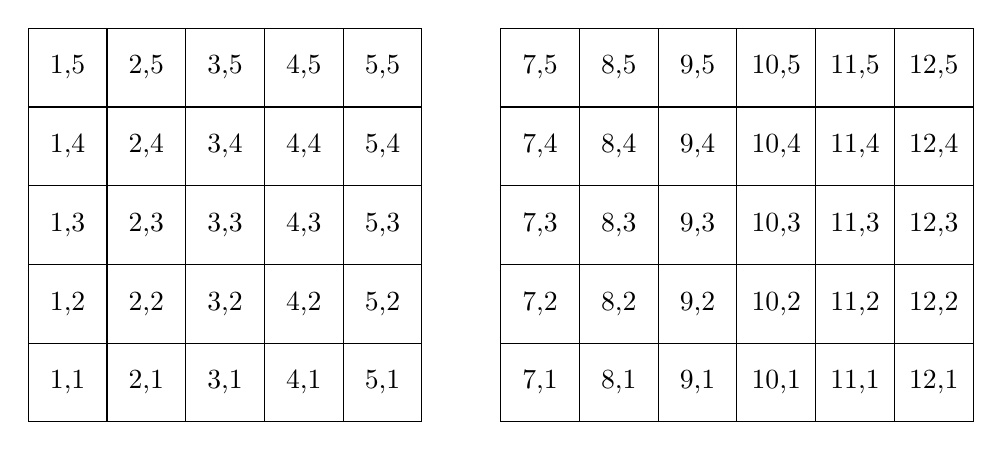
\begin{tikzpicture}
  \foreach \x in {1,2,...,5,7,8,...,12}
    \foreach \y in {1,...,5}
    {
      \draw (\x,\y) +(-.5,-.5) rectangle ++(.5,.5);
      \draw (\x,\y) node{\x,\y};
    }
\end{tikzpicture}
\end{codeexample}

The |\foreach| statement can do even trickier stuff, but the above gives the
idea.


\subsection{Adding Text}

Karl is, by now, quite satisfied with the picture. However, the most important
parts, namely the labels, are still missing!

\tikzname\ offers an easy-to-use and powerful system for adding text and, more
generally, complex shapes to a picture at specific positions. The basic idea is
the following: When \tikzname\ is constructing a path and encounters the
keyword |node| in the middle of a path, it reads a \emph{node specification}.
The keyword |node| is typically followed by some options and then some text
between curly braces. This text is put inside a normal \TeX\ box (if the node
specification directly follows a coordinate, which is usually the case,
\tikzname\ is able to perform some magic so that it is even possible to use
verbatim text inside the boxes) and then placed at the current position, that
is, at the last specified position (possibly shifted a bit, according to the
given options). However, all nodes are drawn only after the path has been
completely drawn/filled/shaded/clipped/whatever.
%
\begin{codeexample}[]
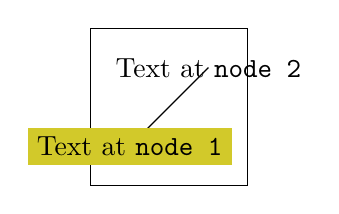
\begin{tikzpicture}
  \draw (0,0) rectangle (2,2);
  \draw (0.5,0.5) node [fill=yellow!80!black]
                       {Text at \verb!node 1!}
     -- (1.5,1.5) node {Text at \verb!node 2!};
\end{tikzpicture}
\end{codeexample}

Obviously, Karl would not only like to place nodes \emph{on} the last specified
position, but also to the left or the right of these positions. For this, every
node object that you put in your picture is equipped with several
\emph{anchors}. For example, the |north| anchor is in the middle at the upper
end of the shape, the |south| anchor is at the bottom and the |north east|
anchor is in the upper right corner. When you give the option |anchor=north|,
the text will be placed such that this northern anchor will lie on the current
position and the text is, thus, below the current position. Karl uses this to
draw the ticks as follows:
%
\begin{codeexample}[]
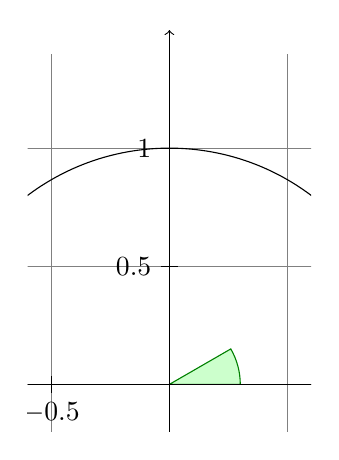
\begin{tikzpicture}[scale=3]
  \clip (-0.6,-0.2) rectangle (0.6,1.51);
  \draw[step=.5cm,help lines] (-1.4,-1.4) grid (1.4,1.4);
  \filldraw[fill=green!20,draw=green!50!black] (0,0) -- (3mm,0mm)
    arc [start angle=0, end angle=30, radius=3mm] -- cycle;
  \draw[->] (-1.5,0) -- (1.5,0);   \draw[->] (0,-1.5) -- (0,1.5);
  \draw (0,0) circle [radius=1cm];

  \foreach \x in {-1,-0.5,1}
    \draw (\x cm,1pt) -- (\x cm,-1pt) node[anchor=north] {$\x$};
  \foreach \y in {-1,-0.5,0.5,1}
    \draw (1pt,\y cm) -- (-1pt,\y cm) node[anchor=east] {$\y$};
\end{tikzpicture}
\end{codeexample}

This is quite nice, already. Using these anchors, Karl can now add most of the
other text elements. However, Karl thinks that, though ``correct'', it is quite
counter-intuitive that in order to place something \emph{below} a given point,
he has to use the \emph{north} anchor. For this reason, there is an option
called |below|, which does the same as |anchor=north|. Similarly, |above right|
does the same as |anchor=south west|. In addition, |below| takes an optional
dimension argument. If given, the shape will additionally be shifted downwards
by the given amount. So, |below=1pt| can be used to put a text label below some
point and, additionally shift it  1pt downwards.

Karl is not quite satisfied with the ticks. He would like to have $1/2$ or
$\frac{1}{2}$ shown instead of $0.5$, partly to show off the nice capabilities
of \TeX\ and \tikzname, partly because for positions like $1/3$ or $\pi$ it is
certainly very much preferable to have the ``mathematical'' tick there instead
of just the ``numeric'' tick. His students, on the other hand, prefer $0.5$
over $1/2$ since they are not too fond of fractions in general.

Karl now faces a problem: For the |\foreach| statement, the position |\x|
should still be given as |0.5| since \tikzname\ will not know where
|\frac{1}{2}| is supposed to be. On the other hand, the typeset text should
really be  |\frac{1}{2}|. To solve this problem, |\foreach| offers a special
syntax: Instead of having one variable |\x|, Karl can specify two (or even
more) variables separated by a slash as in |\x / \xtext|. Then, the elements in
the set over which |\foreach| iterates must also be of the form
\meta{first}|/|\meta{second}. In each iteration, |\x| will be set to
\meta{first} and |\xtext| will be set to \meta{second}. If no \meta{second} is
given, the \meta{first} will be used again. So, here is the new code for the
ticks:
%
\begin{codeexample}[]
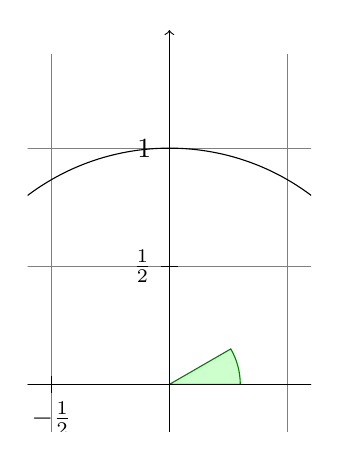
\begin{tikzpicture}[scale=3]
  \clip (-0.6,-0.2) rectangle (0.6,1.51);
  \draw[step=.5cm,help lines] (-1.4,-1.4) grid (1.4,1.4);
  \filldraw[fill=green!20,draw=green!50!black] (0,0) -- (3mm,0mm)
      arc [start angle=0, end angle=30, radius=3mm] -- cycle;
  \draw[->] (-1.5,0) -- (1.5,0); \draw[->] (0,-1.5) -- (0,1.5);
  \draw (0,0) circle [radius=1cm];

  \foreach \x/\xtext in {-1, -0.5/-\frac{1}{2}, 1}
    \draw (\x cm,1pt) -- (\x cm,-1pt) node[anchor=north] {$\xtext$};
  \foreach \y/\ytext in {-1, -0.5/-\frac{1}{2}, 0.5/\frac{1}{2}, 1}
    \draw (1pt,\y cm) -- (-1pt,\y cm) node[anchor=east] {$\ytext$};
\end{tikzpicture}
\end{codeexample}

Karl is quite pleased with the result, but his son points out that this is
still not perfectly satisfactory: The grid and the circle interfere with the
numbers and decrease their legibility. Karl is not very concerned by this (his
students do not even notice), but his son insists that there is an easy
solution: Karl can add the |[fill=white]| option to fill out the background of
the text shape with a white color.

The next thing Karl wants to do is to add the labels like $\sin \alpha$. For
this, he would like to place a label ``in the middle of the line''. To do so,
instead of specifying the label |node {$\sin\alpha$}|  directly after one of
the endpoints of the line (which would place the label at that endpoint), Karl
can give the label directly after the |--|, before the coordinate. By default,
this places the label in the middle of the line, but the |pos=| options can be
used to modify this. Also, options like |near start| and |near end| can be used
to modify this position:
%
\begin{codeexample}[preamble={\usetikzlibrary{intersections}}]
\begin{tikzpicture}[scale=3]
  \clip (-2,-0.2) rectangle (2,0.8);
  \draw[step=.5cm,gray,very thin] (-1.4,-1.4) grid (1.4,1.4);
  \filldraw[fill=green!20,draw=green!50!black] (0,0) -- (3mm,0mm)
    arc [start angle=0, end angle=30, radius=3mm] -- cycle;
  \draw[->] (-1.5,0) -- (1.5,0) coordinate (x axis);
  \draw[->] (0,-1.5) -- (0,1.5) coordinate (y axis);
  \draw (0,0) circle [radius=1cm];

  \draw[very thick,red]
    (30:1cm) -- node[left=1pt,fill=white] {$\sin \alpha$} (30:1cm |- x axis);
  \draw[very thick,blue]
    (30:1cm |- x axis) -- node[below=2pt,fill=white] {$\cos \alpha$} (0,0);
  \path [name path=upward line] (1,0) -- (1,1);
  \path [name path=sloped line] (0,0) -- (30:1.5cm);
  \draw [name intersections={of=upward line and sloped line, by=t}]
    [very thick,orange] (1,0) -- node [right=1pt,fill=white]
    {$\displaystyle \tan \alpha \color{black}=
      \frac{{\color{red}\sin \alpha}}{\color{blue}\cos \alpha}$} (t);

  \draw (0,0) -- (t);

  \foreach \x/\xtext in {-1, -0.5/-\frac{1}{2}, 1}
    \draw (\x cm,1pt) -- (\x cm,-1pt) node[anchor=north,fill=white] {$\xtext$};
  \foreach \y/\ytext in {-1, -0.5/-\frac{1}{2}, 0.5/\frac{1}{2}, 1}
    \draw (1pt,\y cm) -- (-1pt,\y cm) node[anchor=east,fill=white] {$\ytext$};
\end{tikzpicture}
\end{codeexample}

You can also position labels on curves and, by adding the |sloped| option, have
them rotated such that they match the line's slope. Here is an example:
%
\begin{codeexample}[]
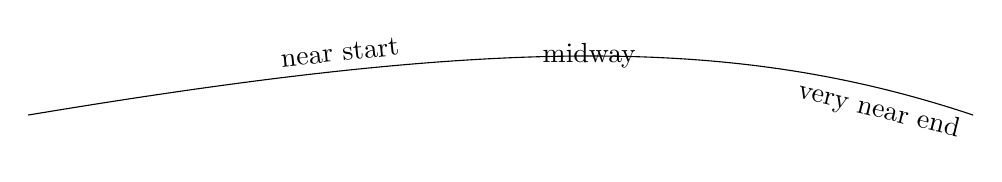
\begin{tikzpicture}
  \draw (0,0) .. controls (6,1) and (9,1) ..
    node[near start,sloped,above] {near start}
    node {midway}
    node[very near end,sloped,below] {very near end} (12,0);
\end{tikzpicture}
\end{codeexample}

It remains to draw the explanatory text at the right of the picture. The main
difficulty here lies in limiting the width of the text ``label'', which is
quite long, so that line breaking is used. Fortunately, Karl can use the option
|text width=6cm| to get the desired effect. So, here is the full code:
%
\begin{codeexample}[code only]
\begin{tikzpicture}
  [scale=3,line cap=round,
  % Styles
  axes/.style=,
  important line/.style={very thick},
  information text/.style={rounded corners,fill=red!10,inner sep=1ex}]

  % Colors
  \colorlet{anglecolor}{green!50!black}
  \colorlet{sincolor}{red}
  \colorlet{tancolor}{orange!80!black}
  \colorlet{coscolor}{blue}

  % The graphic
  \draw[help lines,step=0.5cm] (-1.4,-1.4) grid (1.4,1.4);

  \draw (0,0) circle [radius=1cm];

  \begin{scope}[axes]
    \draw[->] (-1.5,0) -- (1.5,0) node[right] {$x$} coordinate(x axis);
    \draw[->] (0,-1.5) -- (0,1.5) node[above] {$y$} coordinate(y axis);

    \foreach \x/\xtext in {-1, -.5/-\frac{1}{2}, 1}
      \draw[xshift=\x cm] (0pt,1pt) -- (0pt,-1pt) node[below,fill=white] {$\xtext$};

    \foreach \y/\ytext in {-1, -.5/-\frac{1}{2}, .5/\frac{1}{2}, 1}
      \draw[yshift=\y cm] (1pt,0pt) -- (-1pt,0pt) node[left,fill=white] {$\ytext$};
  \end{scope}

  \filldraw[fill=green!20,draw=anglecolor] (0,0) -- (3mm,0pt)
    arc [start angle=0, end angle=30, radius=3mm];
  \draw (15:2mm) node[anglecolor] {$\alpha$};

  \draw[important line,sincolor]
    (30:1cm) -- node[left=1pt,fill=white] {$\sin \alpha$} (30:1cm |- x axis);

  \draw[important line,coscolor]
    (30:1cm |- x axis) -- node[below=2pt,fill=white] {$\cos \alpha$} (0,0);

  \path [name path=upward line] (1,0) -- (1,1);
  \path [name path=sloped line] (0,0) -- (30:1.5cm);
  \draw [name intersections={of=upward line and sloped line, by=t}]
    [very thick,orange] (1,0) -- node [right=1pt,fill=white]
    {$\displaystyle \tan \alpha \color{black}=
      \frac{{\color{red}\sin \alpha}}{\color{blue}\cos \alpha}$} (t);

  \draw (0,0) -- (t);

  \draw[xshift=1.85cm]
    node[right,text width=6cm,information text]
    {
      The {\color{anglecolor} angle $\alpha$} is $30^\circ$ in the
      example ($\pi/6$ in radians). The {\color{sincolor}sine of
        $\alpha$}, which is the height of the red line, is
      \[
      {\color{sincolor} \sin \alpha} = 1/2.
      \]
      By the Theorem of Pythagoras ...
    };
\end{tikzpicture}
\end{codeexample}


\subsection{Pics: The Angle Revisited}

Karl expects that the code of certain parts of the picture he created might be
so useful that he might wish to reuse them in the future. A natural thing to do
is to create \TeX\ macros that store the code he wishes to reuse. However,
\tikzname\ offers another way that is integrated directly into its parser:
pics!

A ``pic'' is ``not quite a full picture'', hence the short name. The idea is
that a pic is simply some code that you can add to a picture at different
places using the |pic| command whose syntax is almost identical to the |node|
command. The main difference is that instead of specifying some text in curly
braces that should be shown, you specify the name of a predefined picture that
should be shown.

Defining new pics is easy enough, see Section~\ref{section-pics}, but right now
we just want to use one such predefined pic: the |angle| pic. As the name
suggests, it is a small drawing of an angle consisting of a little wedge and an
arc together with some text (Karl needs to load the |angles| library and the
|quotes| for the following examples). What makes this pic useful is the fact
that the size of the wedge will be computed automatically.

The |angle| pic draws an angle between the two lines $BA$ and $BC$, where $A$,
$B$, and $C$ are three coordinates. In our case, $B$ is the origin, $A$ is
somewhere on the $x$-axis and $C$ is somewhere on a line at $30^\circ$.
%
\begin{codeexample}[preamble={\usetikzlibrary{angles,quotes}}]
\begin{tikzpicture}[scale=3]
  \coordinate (A) at (1,0);
  \coordinate (B) at (0,0);
  \coordinate (C) at (30:1cm);

  \draw (A) -- (B) -- (C)
        pic [draw=green!50!black, fill=green!20, angle radius=9mm,
             "$\alpha$"] {angle = A--B--C};
\end{tikzpicture}
\end{codeexample}

Let us see, what is happening here. First we have specified three
\emph{coordinates} using the |\coordinate| command. It allows us to name a
specific coordinate in the picture. Then comes something that starts as a
normal |\draw|, but then comes the |pic| command. This command gets lots of
options and, in curly braces, comes the most important point: We specify that
we want to add an |angle| pic and this angle should be between the points we
named |A|, |B|, and |C| (we could use other names). Note that the text that we
want to be shown in the pic is specified in quotes inside the options of the
|pic|, not inside the curly braces.

To learn more about pics, please see Section~\ref{section-pics}.
